This chapter describes how to simulate from our multiGLMM, and describes
a real-based dataset used as an application example. The simulation
procedure is addressed in \autoref{cap:simu}. In \autoref{cap:data} a
simulated dataset based on the Nordic Cancer Union (NCU) twins data is
presented as an application example.

\section{SIMULATING FROM THE MODEL}
\label{cap:simu}

Being able to simulate data from a model is a key task, fundamental to
assess the finite-sample properties and the estimation procedure
liability of a given statistical model. The step-by-step describing the
simulation procedure of our multiGLMM is presented on Algorithm
\autoref{alg:algo}, following the model hierarchical structure
stipulated in Formula \autoref{eq:model}.

\begin{algorithm}[H]
 \caption{SIMULATING FROM A \(\text{multiGLMM}\) FOR CLUSTERED COMPETING
          RISKS DATA}
 \label{alg:algo}
 \begin{algorithmic}[1]
  \State
   Set \(J\), the number of clusters
  \State
   Set \(n_{j}\), the number of cluster elements
   \Comment{can be of different sizes}
  \State
   Set \(K-1\), the number of competing causes of failure
  \State
   Set the model parameter values \(\bm{\theta} =
   [\bm{\beta}~\bm{\gamma}~\bm{w}~\bm{\sigma^{2}}~\bm{\varrho}]^{\top}\)
  \State
   Sample \(J\) latent effect vectors from a
   \(\mathcal{N}_{(K-1)\times(K-1)}(\bm{0},~\Sigma(\bm{\sigma^{2}},
     \bm{\varrho}))\)
  \State
   Set \(\delta\)
   \Comment{maximum follow-up time}
  \State
   Set the failure times \(t_{ij}\)
  \State
   Compute the competing risks probabilities
   \begin{align*}
      p_{kijt}
      &= \frac{\exp\{\bm{x}_{kij}\bm{\beta}_{ki} + u_{kj}\}}{
        1 +
        \sum_{m=1}^{K-1}\exp\{\bm{x}_{mij}\bm{\beta}_{mi} + u_{mj}\}}\\
      &\times
        w_{k}\frac{\delta}{2\delta t - 2t^{2}}~
        \phi\left(
        w_{k}
        \text{arctanh}\left(\frac{t-\delta/2}{\delta/2}\right)
        - \bm{x}_{kij}\bm{\gamma}_{ki} - \eta_{kj}
        \right),\\
      p_{Kijt}
      &= 1 - \sum_{k = 1}^{K - 1} p_{kijt}, \quad k = 1,~2,~\dots,~K -1
    \end{align*}
    \State
    Sample \(J\times n_{j}\) vectors from a
    \(\text{Multinomial}(p_{1ijt},~p_{2ijt},~\dots,~p_{Kijt})\)
    \State
    If \(t_{kij} = \delta\), subject moves to class K
    \Comment{any failure at time \(\delta\) is censored}
    \State
    \Return
    To each individual, its failure/censoring time and from which
    cause-specific it is
  \end{algorithmic}
\end{algorithm}
\vspace{-1cm}
\begin{footnotesize}
  \begin{center}
    SOURCE: The author (2021).
  \end{center}
\end{footnotesize}

Sample \(\varsigma\sim\text{U}(0,~1)\)

Compute the cause-specific failure times by solving
\[
 \varsigma = \Phi[w_{k} g(t_{k}) - X^{\top}\gamma_{k} - \eta_{k}]
 \quad\text{for } t_{k}, \quad k = 1,~2,~\dots,~K - 1
\]

The model described in \autoref{eq:model} is in its most general form,
i.e. allowing for multiple measures at each subject and varying
coefficients. However, we focus on a simpler structure without
covariates, a single measure per subject, and common coefficients.
Putting in practice Algorithm \autoref{alg:algo}, we use the following
model configuration

\begin{align}
  p_{kijt}
  &= \frac{\exp\{\beta_{ki} + u_{kj}\}}{
    1 + \sum_{m=1}^{K-1}\exp\{\beta_{mi} + u_{mj}\}}\nonumber\\
  &\times w_{k}\frac{\delta}{2\delta t - 2t^{2}}~
    \phi\left(
    w_{k}
    \text{arctanh}\left(\frac{t-\delta/2}{\delta/2}\right)
    - \gamma_{ki} - \eta_{kj}
    \right),\quad k = 1,~2,\nonumber\\
  \text{with }\quad
  \bm{\beta}_{i} &= [-2~~~1.5]^{\top}\nonumber\\
  \bm{\gamma}_{i} &= [1.2~~~1]^{\top}\label{eq:modelconfig}\\
  \bm{w} &= [3~~~5]^{\top}\nonumber\\
  \bm{u}_{j} &= [0~~~0]^{\top}\quad
               \bm{\eta}_{j} = [0~~~0]^{\top}\nonumber.
\end{align}
Based on that we get the cluster-specific CIF's and failure
probabilities, its CIF derivatives (dCIF) w.r.t. time \(t\), presented
respectively in \autoref{fig:datasimucif}.

\begin{figure}[H]
  \setlength{\abovecaptionskip}{.0001pt}
  \caption{CLUSTER-SPECIFIC CUMULATIVE INCIDENCE FUNCTIONS (CIF) AND
    RESPECTIVE DERIVATIVES W.R.T. TIME (\(\text{dCIF}\)) FOR A MODEL
    WITH TWO COMPETING CAUSES OF FAILURE, WITHOUT COVARIATES AND THE
    FOLLOWING CONFIGURATION: \(\beta_{1} = -2\), \(\beta_{2} = -1.5\),
    \(\gamma_{1} = 1.2\), \(\gamma = 1\), \(w_{1} = 3\), \(w_{2} = 5\)
    AND LATENT EFFECTS FIXED AT ZERO}
  \vspace{0.2cm} \centering
  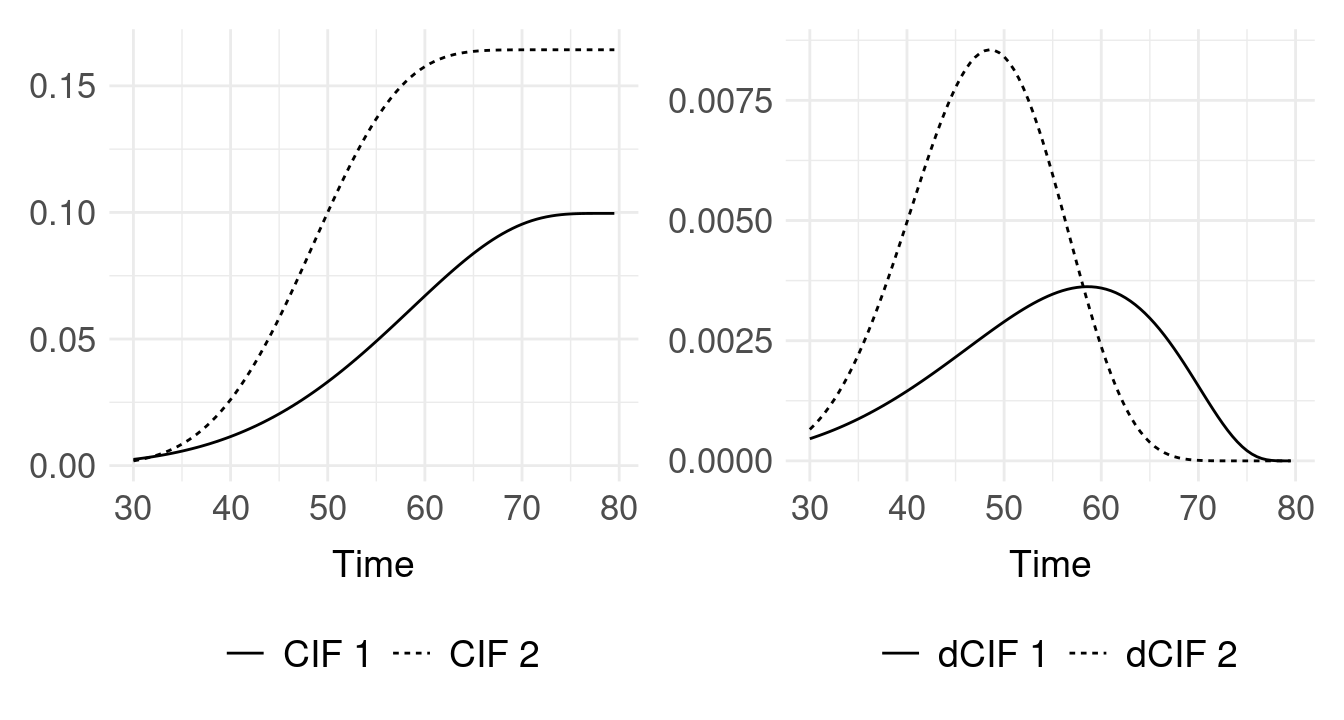
\includegraphics[width=\textwidth]{datasimucif-1.png}
  \\
  \begin{footnotesize}
    SOURCE: The author (2020).
  \end{footnotesize}
  \label{fig:datasimucif}
\end{figure}

By adding the latent structure
\[
  \begin{bmatrix} u_{1}\\u_{2}\\\eta_{1}\\\eta_{2} \end{bmatrix}
  \sim\mathcal{N} \left(
    \begin{bmatrix} 0\\0\\0\\0 \end{bmatrix},
    \begin{bmatrix}
      1&0.4&0.5&0.4\\
      &1&0.4&0.3\\
      &&1&0.4\\
      &&&1
    \end{bmatrix}\right),
\]
in \autoref{eq:modelconfig}, we generate a complete model sample with
500 clusters/pairs of twins, summarized in \autoref{fig:datasimu}.

\begin{figure}[H]
  % \vspace{0.35cm}
  \setlength{\abovecaptionskip}{.0001pt}
  \caption{SUMMARY OF A SIMULATED DATASET WITH 500 PAIRS OF TWINS. A)
    TIME BY TWIN; B) TIMES BOXPLOT; C) PROBABILITIES SCATTERPLOT D)
    \(y_{3}\)'S \%}
  \vspace{0.2cm} \centering
  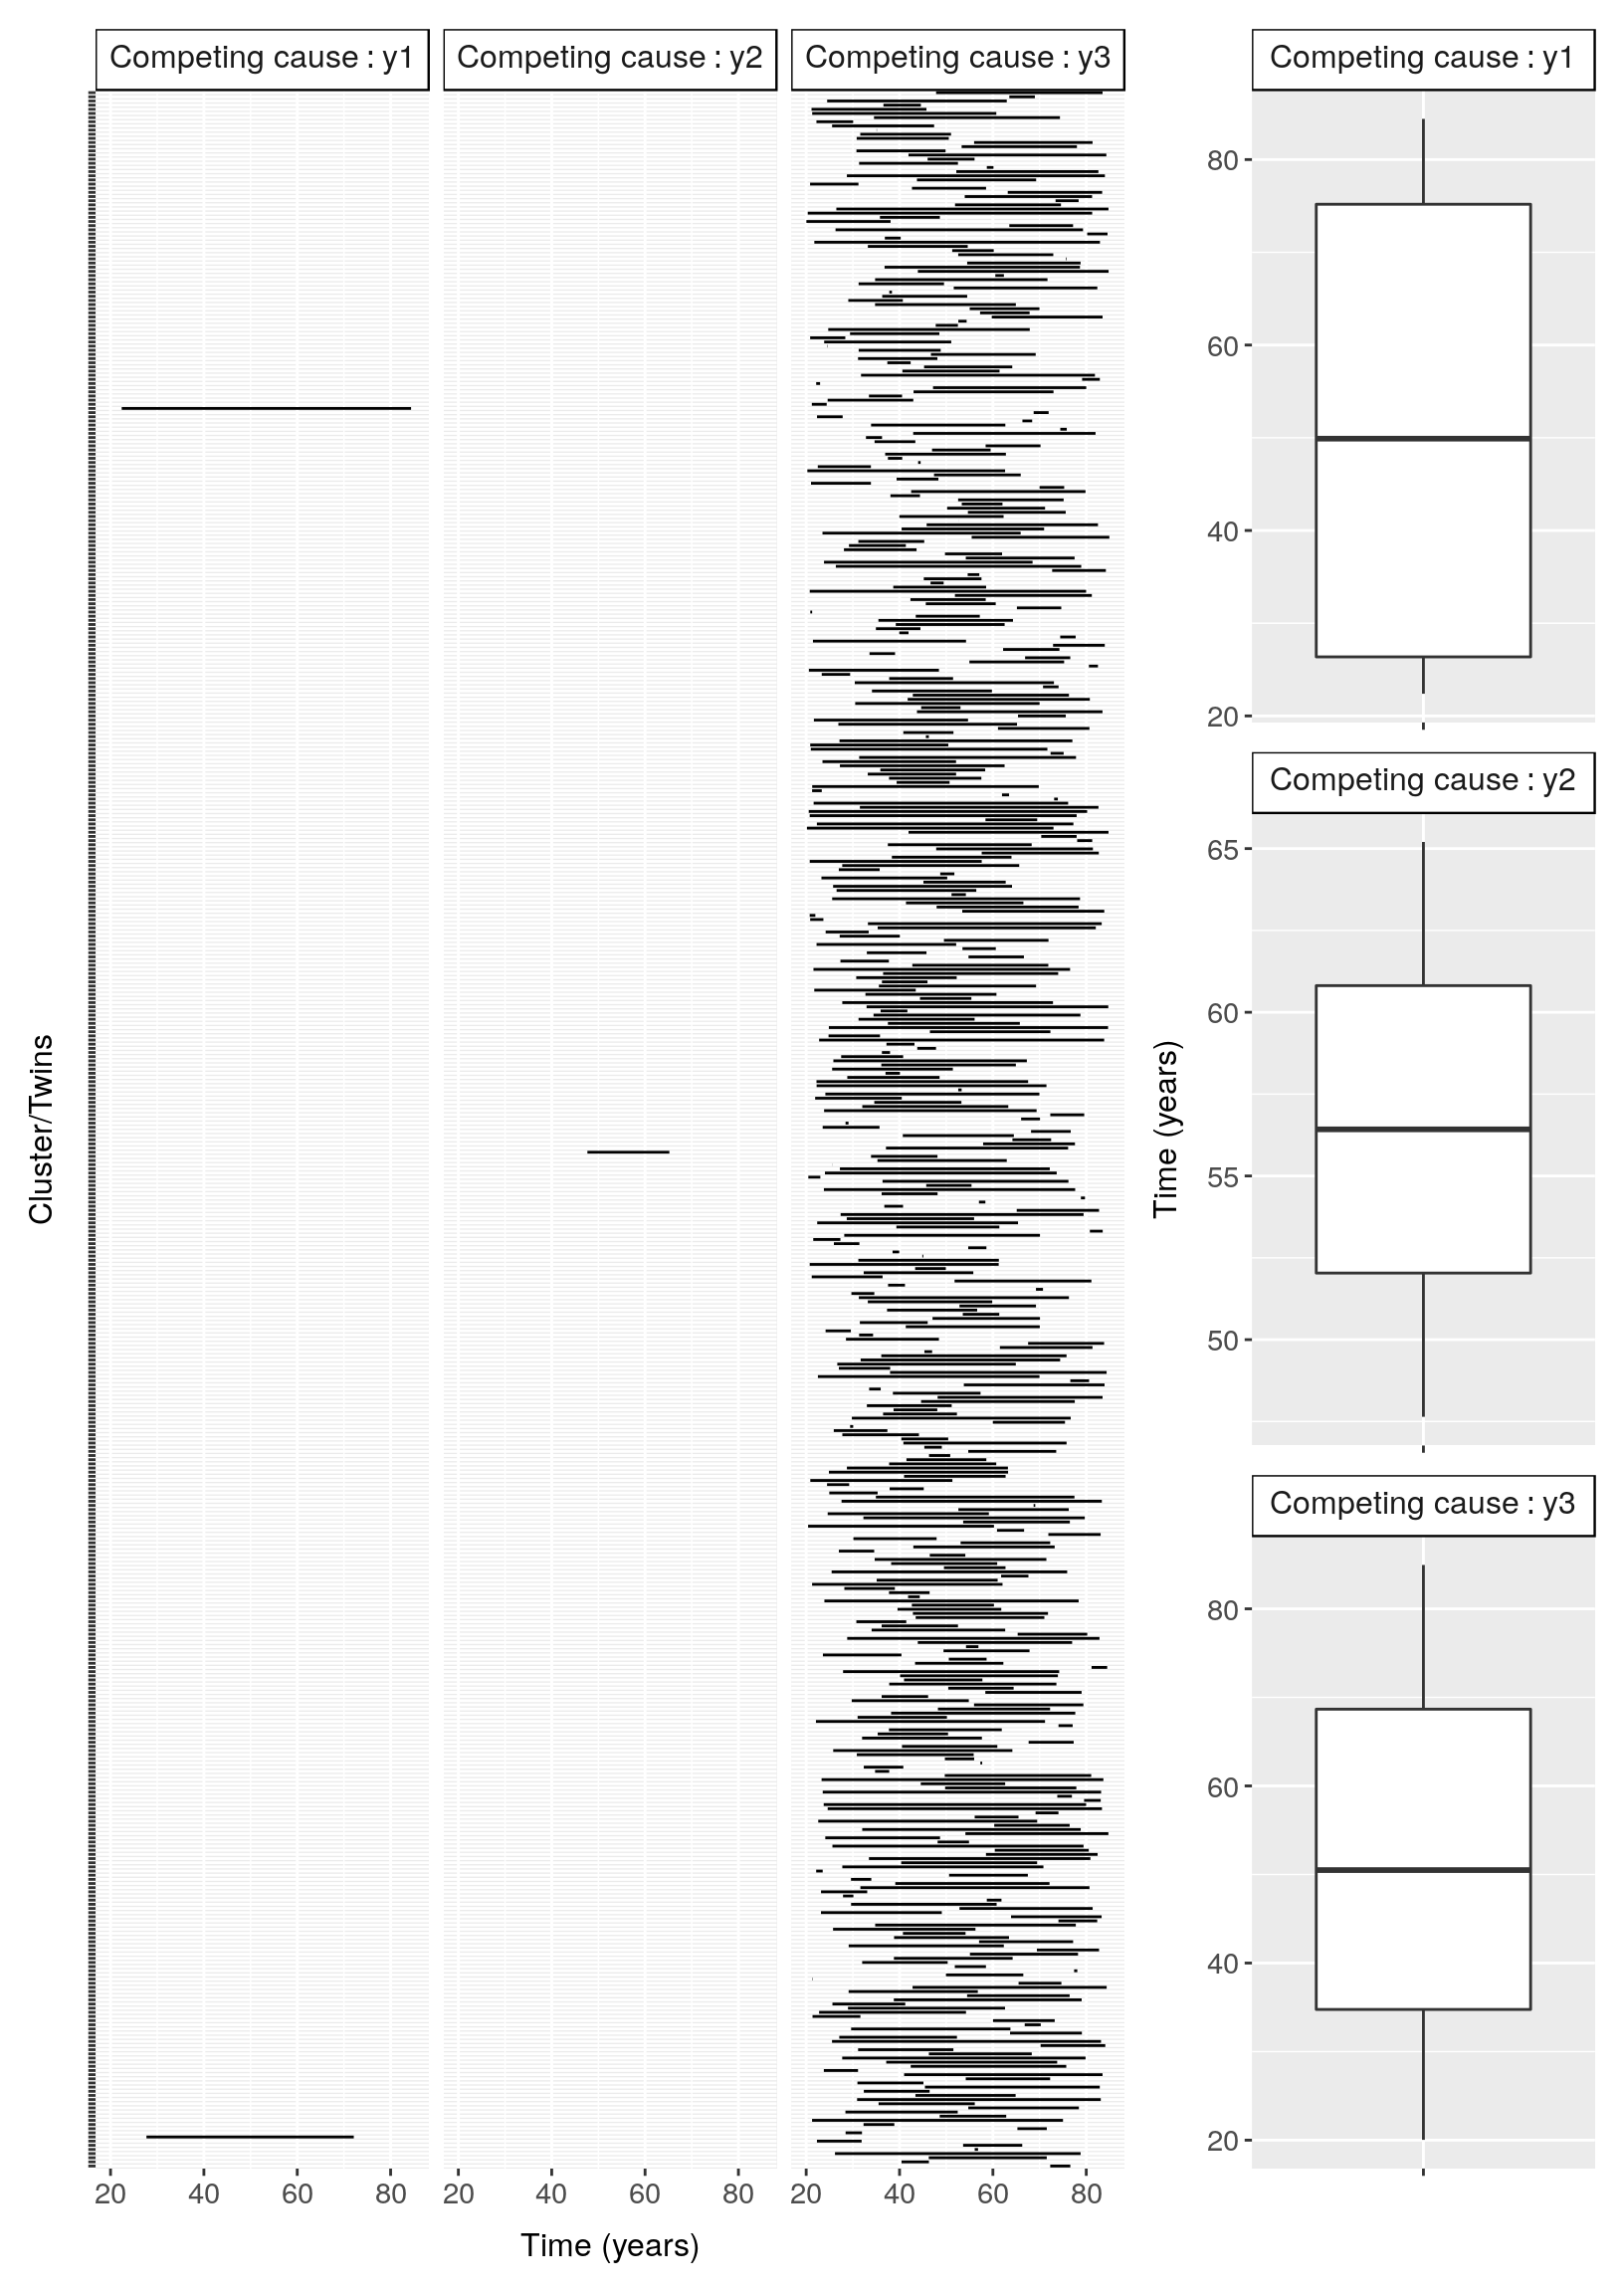
\includegraphics[width=\textwidth]{datasimu-1.png}
  \\
  \vspace{0.2cm}
  \begin{footnotesize}
    SOURCE: The author (2020).
  \end{footnotesize}
  \label{fig:datasimu}
\end{figure}

\section{REAL-BASED DATASET}
\label{cap:data}

% END ==================================================================
